% =================================================================================================
% File:			desc_dp.tex
% Description:	Definisce la sezione relativa all'appendice sui design pattern
% Created:		2015-03-27
% Author:		Tesser Paolo
% Email:		tesser.paolo@mashup-unipd.it
% =================================================================================================
% Modification History:
% Version		Modifier Date		Change											Author
% 0.0.1 		2015-03-27 			creato scheletro								Tesser Paolo
% =================================================================================================
% 0.0.2			2015-04-10			aggiunto scheltro per altri DP trovati			Tesser Paolo
% =================================================================================================
%

% CONTENUTO DEL CAPITOLO



\section{Descrizione Design Pattern} % (fold)
\label{sec:descdp}
	\subsection{Design pattern architetturali} % (fold)

		\subsubsection{Three-Tier} % (fold)
		
		
		\begin{figure}[htbp]
			\centering
			\centerline{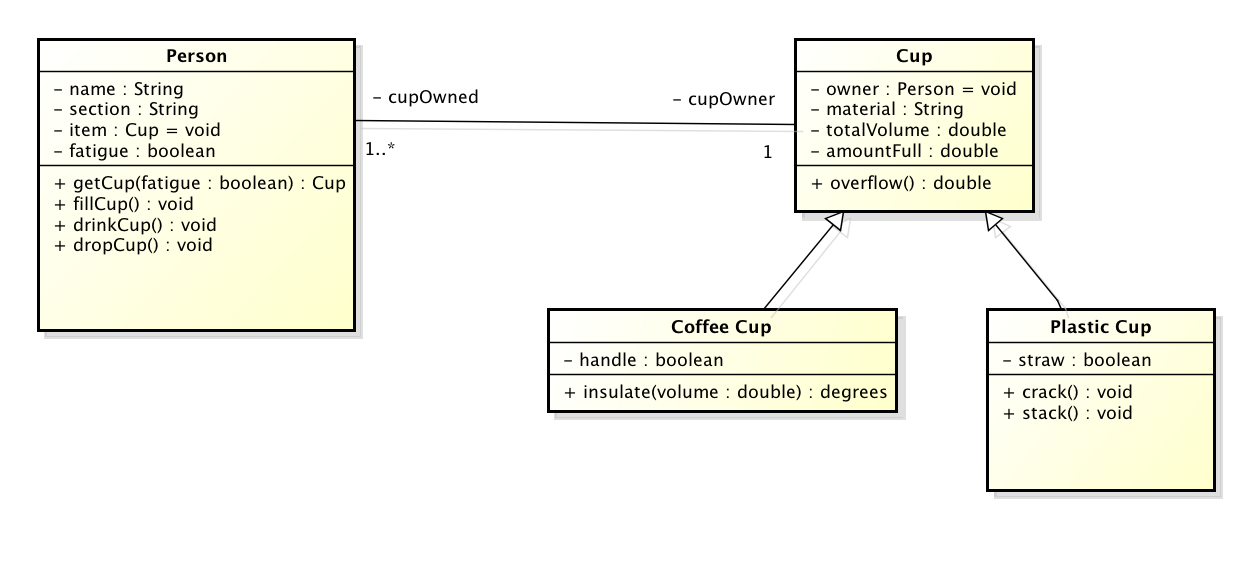
\includegraphics[scale=0.3]{./images/example_graph.png}}
			\caption{Design pattern architetturale - Three-Tier}
		\end{figure}
		TO DO (grafico)
		
		
		\begin{itemize}
			\item \textbf{Scopo}: L'architettura three-tier, detta anche "a tre strati", identifica una particolare architettura software per l'esecuzione di un'applicazione web che prevede la suddivisione dell'applicazione in tre diversi moduli o strati dedicati rispettivamente all'interfaccia utente, alla logica funzionale e alla gestione dei dati persistenti. Tale architettura va tipicamente a mappare a livello fisico-infrastrutturale quella del sistema informatico ospitante l'applicazione da eseguire.
Tali moduli sono intesi interagire fra loro secondo le linee generali del paradigma client-server ( l'interfaccia è cliente della business logic, e questa è cliente del modulo di gestione dei dati persistenti) e utilizzando interfacce ben definite. In questo modo, ciascuno dei tre moduli può essere modificato o sostituito indipendentemente dagli altri conferendo scalabilità e manutenibilità all'applicazione. Nella maggior parte dei casi, i diversi moduli possono essere distribuiti su diversi nodi di una rete anche eterogenea;
			
			\item \textbf{Motivazione}: E' stato scelto questo pattern perchè TO DO;
			
			\item \textbf{Applicabilità}: Questo pattern è stato utilizzato nella progettazione ad alto livello del client dell'applicazione;
			
		\end{itemize}
		% subsubsection three_tier (end)


		\newpage
		\subsubsection{MVC} % (fold)
		
		\begin{figure}[htbp]
			\centering
			\centerline{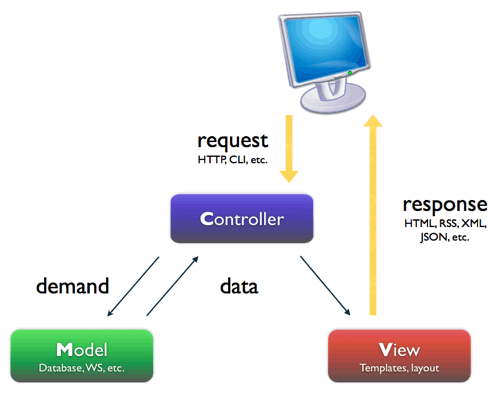
\includegraphics[scale=0.6]{./images/mvc.png}}
			\caption{Design pattern architetturale - MVC}
		\end{figure}
		TO DO (da rifare grafico tramite Astah in maniera che sia conforme agli altri grafici, può essere sempre generale a livello di nomi, ma così viene più elegante)

		\begin{itemize}
			\item \textbf{Scopo}: Il pattern è basato sulla separazione dei compiti fra i componenti software che interpretano tre ruoli principali:
			
		\begin{itemize}
			\item \textbf{Model} che fornisce i metodi per accedere ai dati utili all'applicazione;
			\item \textbf{View} che visualizza i dati contenuti nel model e si occupa dell'interazione con utenti e agenti;
			\item \textbf{Controller} che riceve i comandi dell'utente (in genere attraverso il view) e li attua modificando lo stato degli altri due componenti.
		\end{itemize}
		
		\noindent
		Questo schema implica anche la tradizionale separazione fra la logica applicativa (in questo contesto spesso chiamata ``logica di business''), a carico del controller e del model, e l'interfaccia utente a carico del view. I dettagli delle interazioni fra questi tre oggetti software dipendono molto dalle tecnologie usate (linguaggio di programmazione, eventuali librerie, middleware e via dicendo) e dal tipo di applicazione (per esempio se si tratta di un'applicazione web, o di un'applicazione desktop). Quasi sempre la relazione fra view e model è descrivibile anche come istanza del pattern Observer. A volte, quando è necessario cambiare il comportamento standard dell'applicazione a seconda delle circostanze, il controller implementa anche il pattern Strategy.;
			
			\item \textbf{Motivazione}: E' stato scelto questo pattern perchè TO DO;
			
			\item \textbf{Applicabilità}: Questo pattern è stato utilizzato nella progettazione del client dell'applicazione, in particolare viene implementato dal framework Angular JS nella realizzazione dell'interfaccia utente dell'applicazione;
		\end{itemize}	
				
		
		\newpage
		\subsubsection{MVVM} % (fold)
		
		\begin{figure}[htbp]
			\centering
			\centerline{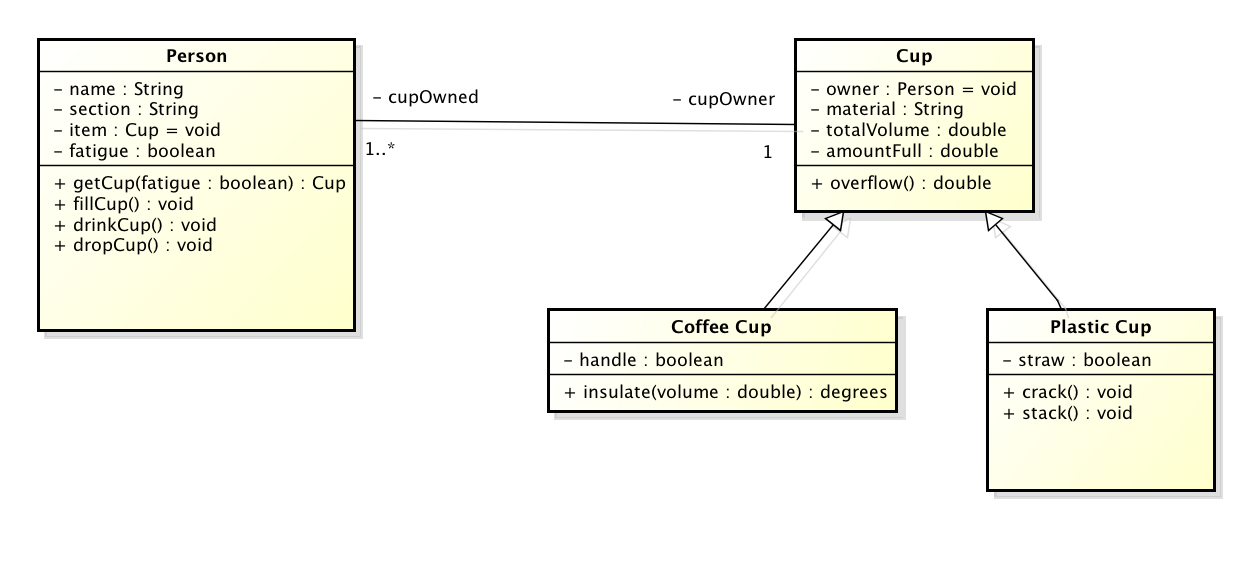
\includegraphics[scale=0.3]{./images/example_graph.png}}
			\caption{Design pattern architetturale - MVVM}
		\end{figure}
		TO DO (grafico)
		
		
		\begin{itemize}
			\item \textbf{Scopo}: E' una variante del pattern MVC. Questo pattern propone un ruolo più attivo della View rispetto a MVC: la View è in grado di gestire eventi, eseguire operazioni ed effettuare il data-binding. In questo contesto, quindi, alcune delle funzionalità del Controller vengono inglobate nella View, la quale si appoggia su un’estensione del Model: il ViewModel.
Il ViewModel è quindi un Model esteso con funzionalità per la manipolazione dei dati e per l’interazione con la View;
			
			\item \textbf{Motivazione}: E' stato scelto questo pattern perchè ha un impatto positivo nella progettazione di interfacce utente e viene implementato in modo semplice da Angular JS;
			
			\item \textbf{Applicabilità}: Questo pattern è stato utilizzato nella progettazione del client dell'applicazione;
			
		\end{itemize}
		
		
		\newpage
		\subsubsection{Dependency Injection} % (fold)
		
		\begin{figure}[htbp]
			\centering
			\centerline{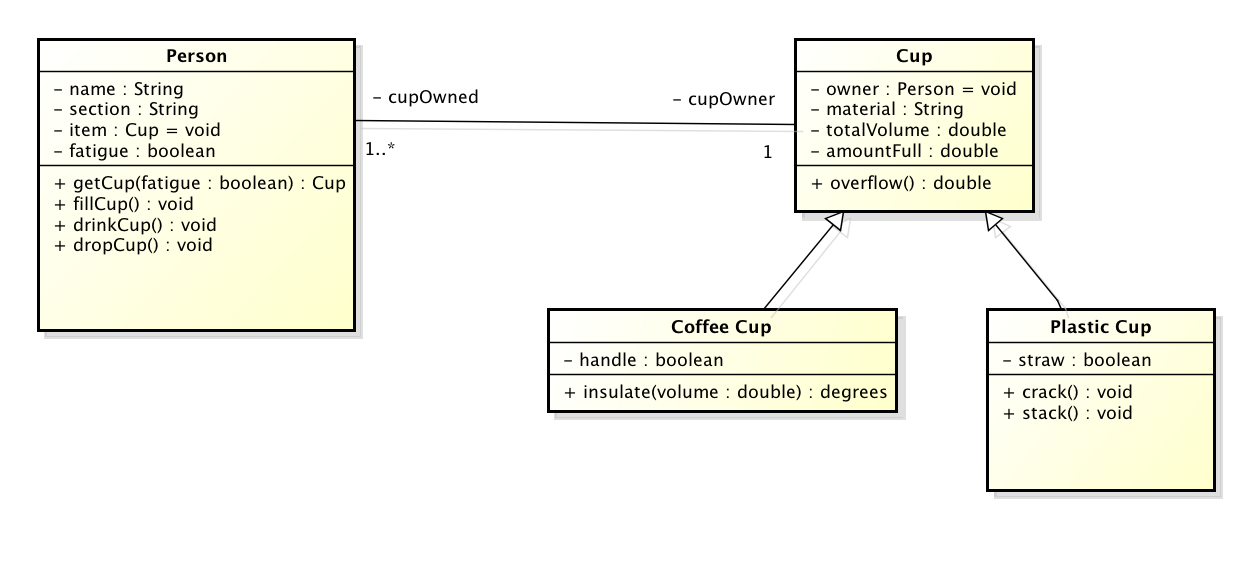
\includegraphics[scale=0.3]{./images/example_graph.png}}
			\caption{Design pattern architetturale - Dependency Injection}
		\end{figure}
		TO DO (grafico)
		
		
		\begin{itemize}
			\item \textbf{Scopo}: è quello di semplificare lo sviluppo e migliorare la testabilità di software di grandi 		dimensioni.
Il pattern Dependency Injection coinvolge almeno tre elementi:

				\begin{itemize}
					\item una componente dipendente;
					\item la dichiarazione delle dipendenze del componente, definite come interface contracts;
					\item un injector (chiamato anche provider o container) che crea, a richiesta, le istanze delle classi che implementano delle dependency interfaces;
				\end{itemize}
			
			\item \textbf{Motivazione}: E' stato scelto questo pattern perchè TO DO;
			
			\item \textbf{Applicabilità}: Questo pattern è stato utilizzato nella progettazione del TO DO;
			
		\end{itemize}
		
	% subsection design_pattern_architetturali (end)


	\clearpage 
	\newpage
	\subsection{Design pattern creazionali} % (fold)
	
		\subsubsection{Prototype Pattern} % (fold)

		\begin{figure}[htbp]
			\centering
			\centerline{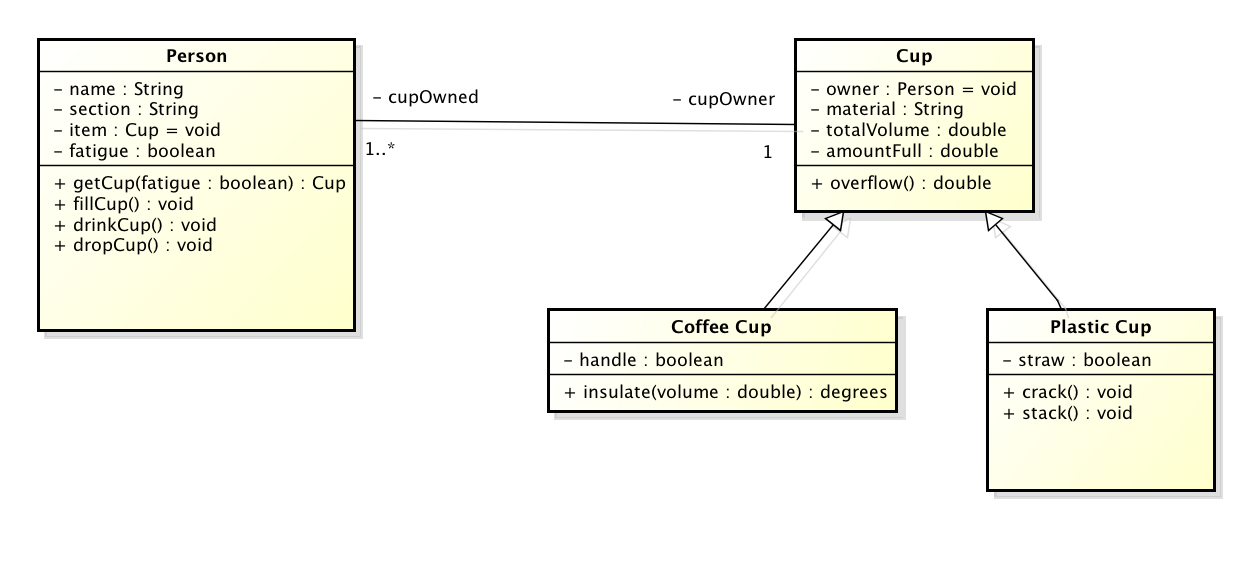
\includegraphics[scale=0.3]{./images/example_graph.png}}
			\caption{Design pattern creazionale - Prototype Pattern}
		\end{figure}
		TO DO (grafico)
		
		
		\begin{itemize}
			\item \textbf{Scopo}: Prototype permette di creare nuovi oggetti clonando un oggetto iniziale, detto appunto prototipo. A differenza di altri pattern come Abstract factory o Factory method permette di specificare nuovi oggetti a tempo d'esecuzione (run-time), utilizzando un gestore di prototipi ( detto prototype manager ) per salvare e reperire dinamicamente le istanze degli oggetti desiderati;
			
			\item \textbf{Motivazione}: E' stato scelto questo pattern perchè permette di incapsulare al suo interno la modalità di istanziazione degli oggetti, liberando il client dalla necessità di conoscere i nomi delle classi da instanziare. Inoltre permette di ridurre la complessità della gerarchia delle sottoclassi rispetto al Factory Method ed evitare la duplicazione di codice quando si usano diverse classi simili tra loro;
			
			\item \textbf{Applicabilità}: Come altri pattern creazionali, Prototype mira a rendere indipendente un sistema dal modo in cui i suoi oggetti vengono creati. Questo pattern è stato utilizzato nella progettazione del componente TO DO dell'applicazione;
			
		\end{itemize}
		% subsubsection prototype_pattern (end)
		
		
		\newpage
		\subsubsection{Module Pattern} % (fold)
		
		
		\begin{figure}[htbp]
			\centering
			\centerline{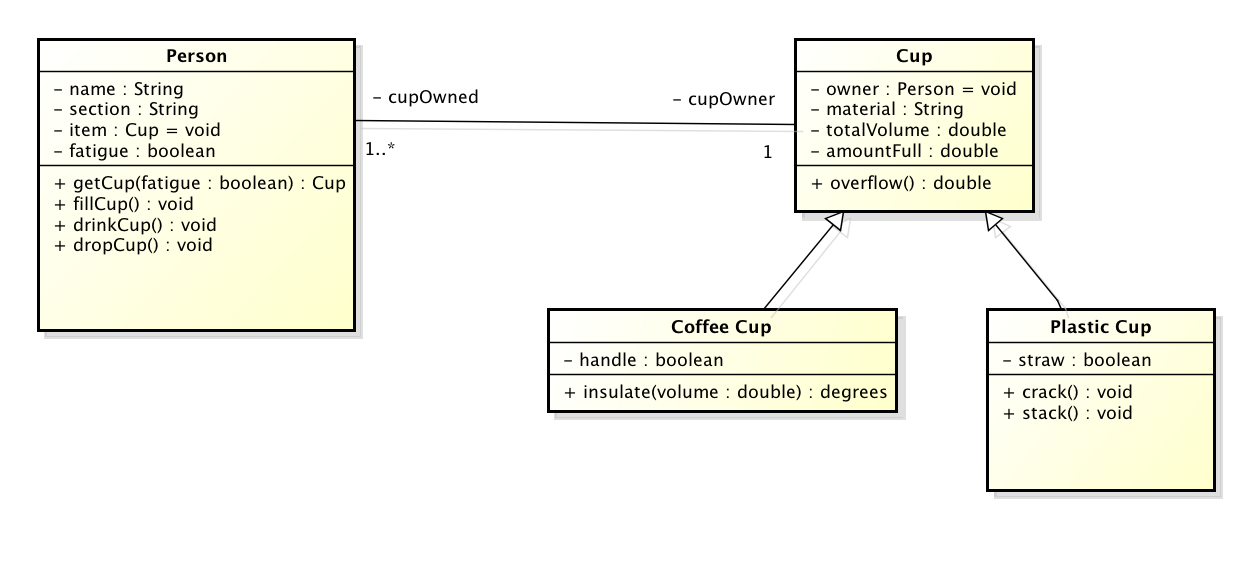
\includegraphics[scale=0.3]{./images/example_graph.png}}
			\caption{Design pattern creazionale - Module Pattern}
		\end{figure}
		TO DO (grafico)
		
		
		\begin{itemize}
			\item \textbf{Scopo}: Il module pattern prevede che l'applicazione che lo implementa sia divisa in moduli funzionali distinti. Essi consentono di organizzare le parti di un’applicazione in unità separate ma integrabili grazie ai meccanismi di esportazione e importazione, cioè rispettivamente della possibilità di rendere pubblicamente accessibile del codice e di accedere a codice esportato da altri moduli;
			
			\item \textbf{Motivazione}: E' stato scelto questo pattern perché permette all'applicazione di essere robusta e facilmente gestibile;
			
			\item \textbf{Applicabilità}: Questo pattern è stato utilizzato nella progettazione del componente TO DO dell'applicazione;
			
		\end{itemize}


		\newpage
		\subsubsection{Singleton} % (fold)
		
		\begin{figure}[htbp]
			\centering
			\centerline{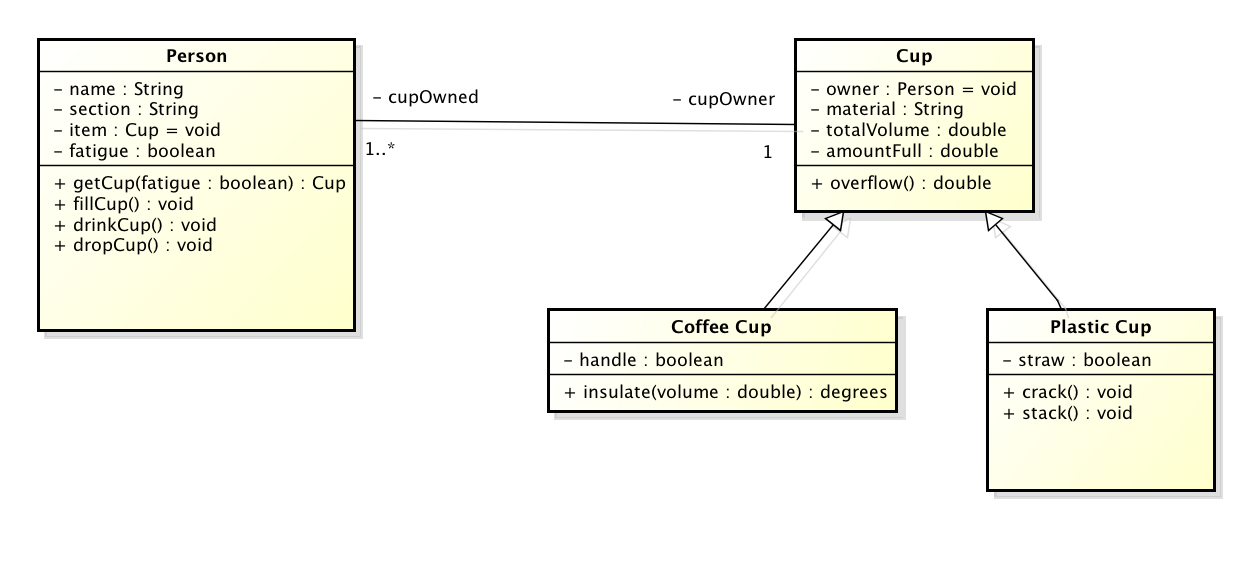
\includegraphics[scale=0.3]{./images/example_graph.png}}
			\caption{Design pattern creazionale - Singleton}
		\end{figure}
		TO DO (grafico)
		
		
		\begin{itemize}
			\item \textbf{Scopo}: Il singleton ha lo scopo di garantire che di una determinata classe venga creata una e una sola istanza, e di fornire un punto di accesso globale a tale istanza;
						
			\item \textbf{Motivazione}: E' stato scelto questo pattern perché si è reso necessario creare istanze uniche di classi all'interno dell'applicazione;
			
			\item \textbf{Applicabilità}: Questo pattern è stato utilizzato nella progettazione del componente TO DO dell'applicazione;
		\end{itemize}
		
		% subsubsection singleton (end)
		% subsubsection module_pattern (end)

	% subsection design_pattern_creazionali (end)


	\clearpage 
	\newpage
	\subsection{Design pattern strutturali} % (fold)
		\subsubsection{Fa\c{c}ade} % (fold)
		
		
		\begin{figure}[htbp]
			\centering
			\centerline{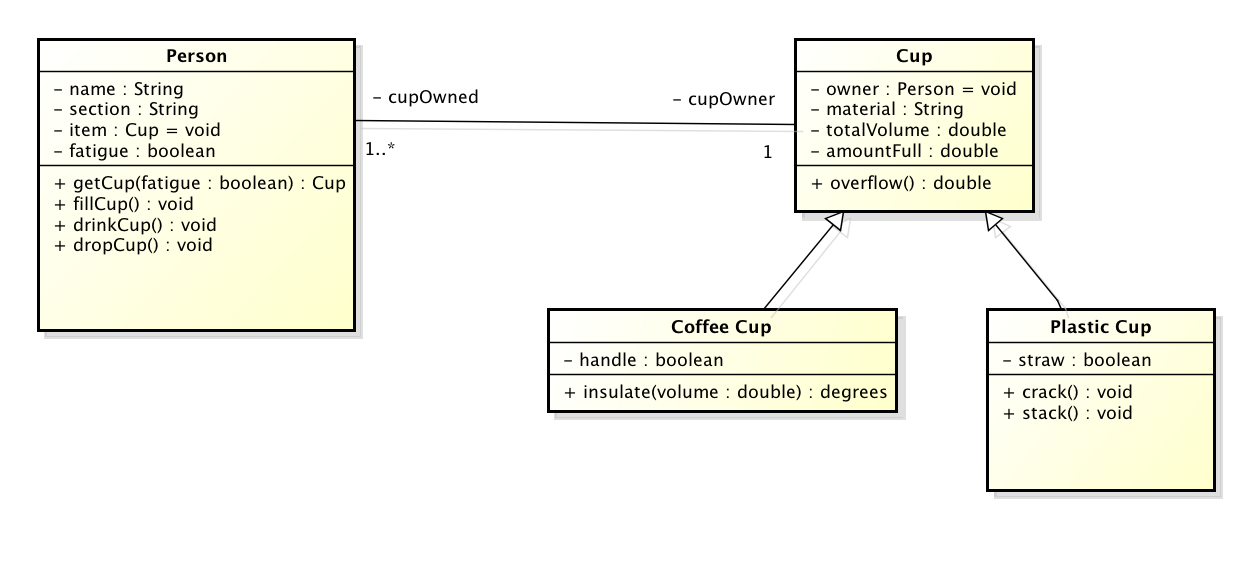
\includegraphics[scale=0.3]{./images/example_graph.png}}
			\caption{Design pattern strutturalie - Fa\c{c}ade}
		\end{figure}
		TO DO (grafico)
		
		
		\begin{itemize}
			\item \textbf{Scopo}: Il "Facade" pattern suggerisce la creazione di un oggetto che presenti un'interfaccia semplificata al cliente, ma in grado di gestire tutta la complessità delle interazioni tra gli oggetti delle diverse classi per compiere l'obbiettivo desiderato;
			
			\item \textbf{Motivazione}: E' stato scelto questo pattern perché fornisce una interfaccia unificata per un insieme di interfacce di un sottosistema, rendendo più facile l'uso di quest'ultimo.;
			
			\item \textbf{Applicabilità}: Questo pattern è stato utilizzato nella progettazione del componente TO DO dell'applicazione;
			
		\end{itemize}



	% subsection design_pattern_strutturali (end)

	\clearpage 
	\newpage
	\subsection{Design pattern comportamentali} % (fold)
		\subsubsection{Page Controller} % (fold)
		
		
		\begin{figure}[htbp]
			\centering
			\centerline{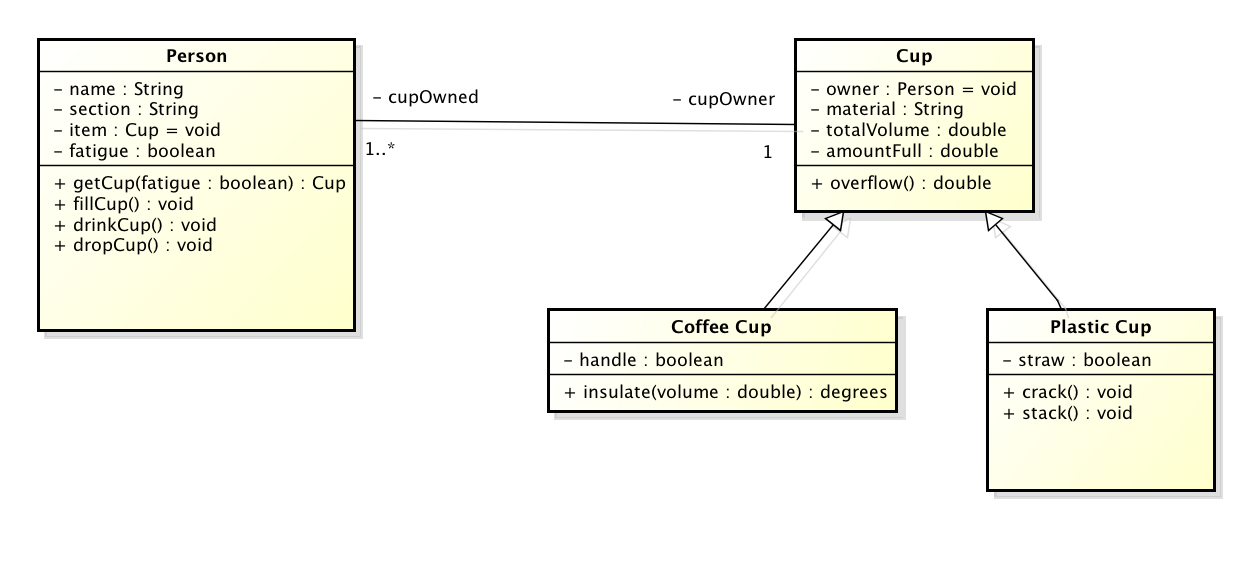
\includegraphics[scale=0.3]{./images/example_graph.png}}
			\caption{Design pattern comportamentale - Page Controller}
		\end{figure}
		TO DO (grafico)
		
		
		\begin{itemize}
			\item \textbf{Scopo}: Il Page Controller pattern suggerisce la creazione di un oggetto dedicato che si occupa di gestire una richiesta per una specifica pagina o azione in un sito Web. Implica quindi che esiste un singolo file che gestisce la richiesta di una specifica pagina. Questo semplice meccanismo rispecchia il funzionamento delle pagine web statiche;
					
			\item \textbf{Motivazione}: E' stato scelto questo pattern perché semplifica la gestione delle pagine web statiche utilizzate dall'applicazione;
			
			\item \textbf{Applicabilità}: Questo pattern è stato utilizzato nella progettazione del componente TO DO dell'applicazione;
			
		\end{itemize}
		% subsubsection page_controller (end)
		
		
		\newpage
		\subsubsection{Template View} % (fold)
		
		
		\begin{figure}[htbp]
			\centering
			\centerline{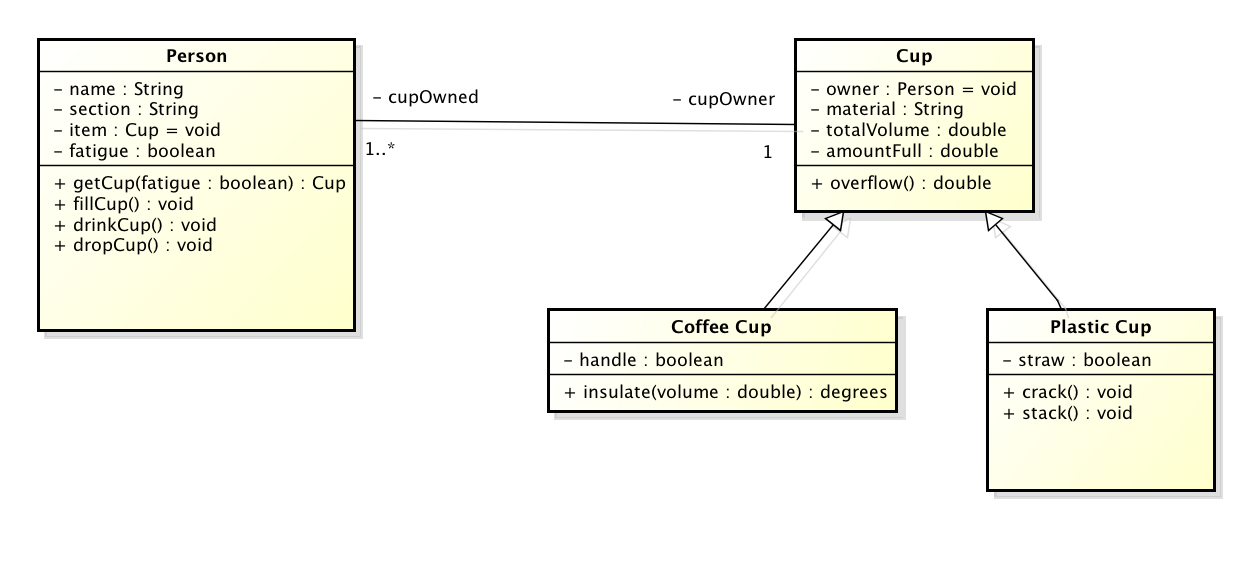
\includegraphics[scale=0.3]{./images/example_graph.png}}
			\caption{Design pattern comportamentale - Template View}
		\end{figure}
		TO DO (grafico)
		
		
		\begin{itemize}
			\item \textbf{Scopo}: Questo pattern specifica la struttura algoritmica di una operazione, demandando l'implementazione di alcuni passi dei suoi metodi alle sottoclassi. Il Template Method consente di ridefinire certi passi di un algoritmo senza cambiare la sua struttura;
			
			\item \textbf{Motivazione}: E' stato scelto questo pattern perché TO DO;
			
			\item \textbf{Applicabilità}: Questo pattern è stato utilizzato nella progettazione del componente TO DO dell'applicazione;
			
		\end{itemize}
		% subsubsection template_view (end)

	% subsection design_pattern_comportamentali (end)


% section descdp (end)